\section{Delaunay triangulatie}
Om verschillende punten mooi te verbinden, kan er gebruik worden gemaakt van een Delaunay triangulatie. Deze triangulatie wordt toegepast op de middenpunten van de schermen. Wanneer deze triangulatie op de schermen wordt geprojecteerd, zullen de liggingen van de schermen mooi worden weergegeven. Bij een Delaunay triangulatie worden alle punten zo verbonden dat ze verscheidene driehoeken vormen. De zijden van de driehoeken mogen niet overlappen en de kleinste hoek in de triangulatie moet gemaximaliseerd worden. \cite{delaunaywiki}

De triangulatie kan op vele manieren worden berekend, in dit verslag zijn er twee soorten algoritmen onderzocht. Het S-hull algoritme en het Boyler-Watson algoritme.

\subsection{S-hull}
Het eerste algoritme is het S-hull algoritme. Het is een $O(nlog(n))$ algoritme, gebruikmakend van een radiaal propagerende sweep hull. S-hull start met twee punten, één daarvan is willekeurig geselecteerd. Het tweede punt is het dichtsbijzijnde. Vervolgens zal er een derde worden gezocht dat samen met de twee voorgaande een zo klein mogelijke cirkel maakt. Het middenpunt van deze cirkel wordt gebruikt om alle punten te sorteren t.o.v. de afstand met het gevonden middenpunt. Deze gesorteerde punten zullen één voor één toegevoegd worden aan de triangulatie.

Nadat ze sequentieel zijn toegevoegd, is er een niet overlappende triangulatie bekomen. Om een Delaunay triangulatie te bekomen moet er echter ook gekeken worden naar de hoeken. Elke driehoek zal nu worden afgegaan en er wordt gekeken of er geen andere driehoek kan gevormd worden met de buurdriehoeken zodat de minimale hoek gemaximaliseerd wordt, zie figuur \ref{driehoekswitch}. \cite{s-hull}
\begin{figure}

	\center
	\begin{subfigure}{0.4\textwidth}
		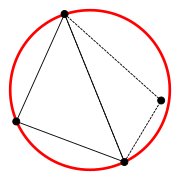
\includegraphics[width=\textwidth]{slechte_driehoek}
		\caption{De twee buurdriehoeken blijken niet ideaal te zijn.}
	\end{subfigure}
	\begin{subfigure}{0.4\textwidth}
		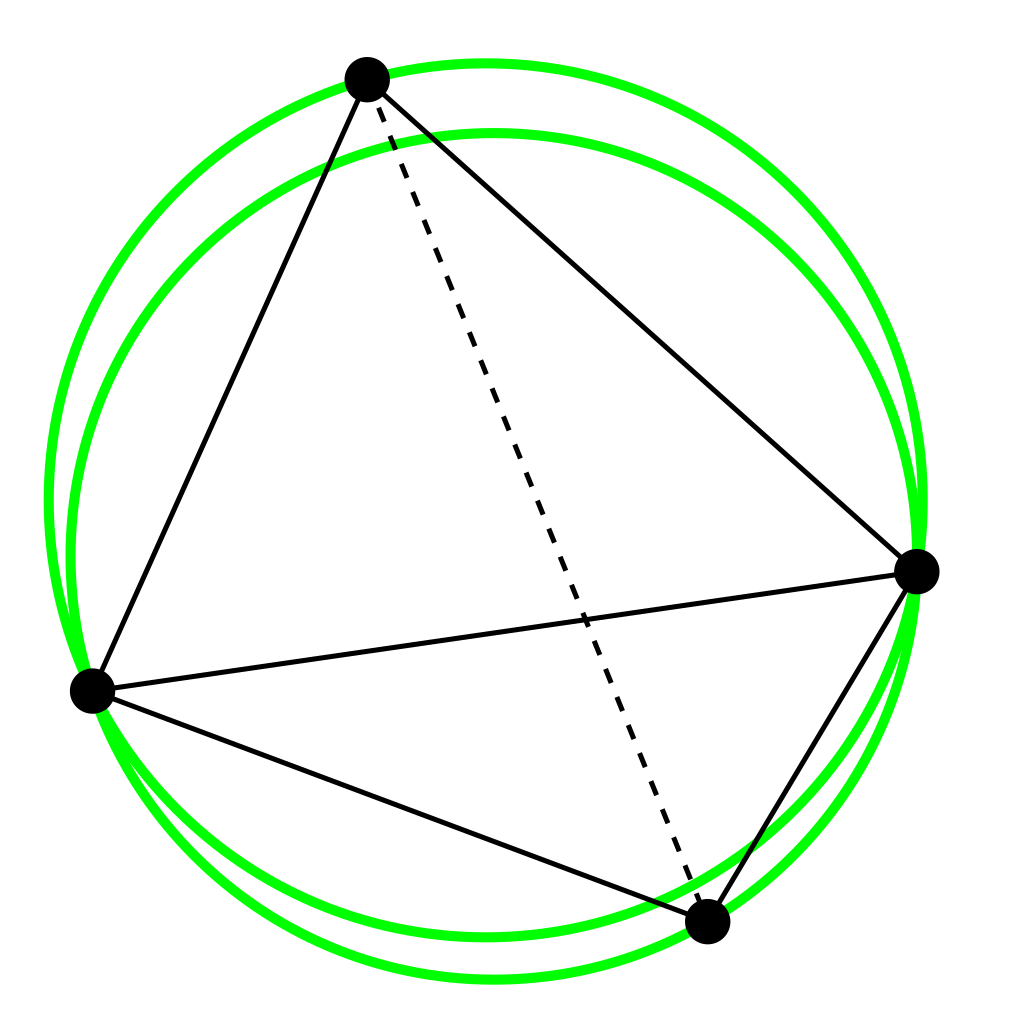
\includegraphics[width=\textwidth]{goede_driehoek}
		\caption{De twee buurdriehoeken maximaliseren met een andere verbinding de kleinste hoek.}
	\end{subfigure}
	\caption{Het maximaliseren van de kleinste hoek \cite{delaunaywiki}}
	\label{driehoekswitch}
\end{figure}

Dit algoritme is echter niet gebruikt. Ook al is het algoritme $O(nlog(n))$ het vereist een zeer goede data management om deze snelheid te behalen.  \cite{Lund2014} Er is daarom gekozen voor een simpeler algoritme, namelijk het Boyler-Watson algoritme.

\subsection{Bowyer-Watson}
Het Bowyer-Watson algoritme is wel geïmplementeerd. Het heeft een tijdscomplexiteit van $O(n^2)$, dit is aanzienlijk trager dan het S-hull algoritme. \cite{Bowyer-WatsonWiki} Het vereist echter een minder complex data management en is daarom ook makkelijker te implementeren. De tijdscomplexiteit is ook relatief te zien, er zijn namelijk maar maximaal detecteerbare 120 schermen. Meer kunnen er door het identificatiemechanisme niet worden gevonden. Gezien het laag aantal punten, moet het algoritme niet nodeloos complex worden en kan er gekeken worden naar `tragere' algoritmen, zoals het Bowyer-Watson algoritme.

\paragraph{}
Bowyer-Watson gaat er van uit dat punten enkel worden toegevoegd in een al bestaande Delaunay triangulatie. Als eerste worden er twee superdriehoeken gezocht. Deze driehoeken zullen alle te trianguleren punten bevatten. De implementaties waarop het algoritme is gebaseerd \cite{Bowyer-WatsonWiki} \cite{bowyer-watsonImplementation} stelden beiden een `superdriehoek' voor, zie figuur \ref{bowyer-watson-a} Echter is het simpeler om een omkaderende vierhoek te vormen en deze te splitsen in twee driehoeken. Vervolgens worden alle punten één voor één toegevoegd.

Voor elk punt worden de driehoeken gezocht waarvan het punt in de omschreven cirkel zit. Wanneer twee driehoeken eenzelfde zijde delen, wordt deze verwijderd. Alle punten van de omschreven veelhoek van de twee driehoeken worden nu verbonden met het toegevoegde punt, zie figuur \ref{bowyer-watson-b}. Met deze werkwijze zal er op elk moment een Delaunay triangulatie zijn en moeten de driehoeken achteraf niet meer overlopen worden. Dit maakt het data management minder complex.

Als alle punten zijn toegevoegd, worden de driehoeken die één of meer hoeken van de omkaderende vierhoek bevatten verwijderd, zie figuur \ref{bowyer-watson-c}. Aangezien deze driehoeken aan de buitenkant liggen is dit toegestaan. Er zal een Delaunay triangulatie overblijven van alle onderzochte punten.

\begin{figure}
	\center
	\begin{subfigure}{0.4\textwidth}
		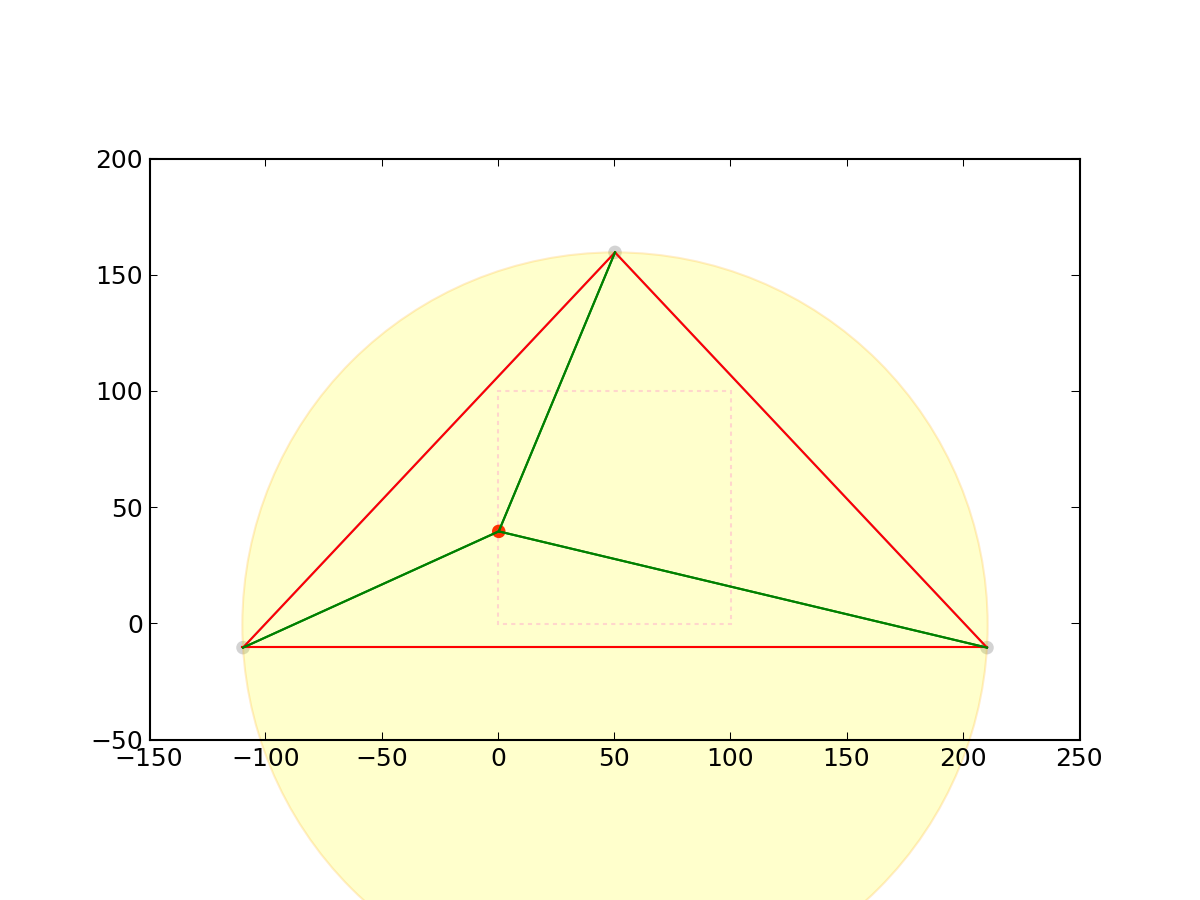
\includegraphics[width=\textwidth]{bowyer-watson_superdriehoek}
		\caption{De rode superdriehoek waarin alle punten zullen worden toegevoegd.}
		\label{bowyer-watson-a}
	\end{subfigure}
	\begin{subfigure}{0.4\textwidth}
		\includegraphics[width=\textwidth]{bowyer-watson_nieuwpunt}
		\caption{Een nieuw punt wordt toegevoegd. In geel de omschreven cirkels. De gestippelde zijde wordt verwijderd, de groenen toegevoegd.}
		\label{bowyer-watson-b}
	\end{subfigure}
		\begin{subfigure}{0.4\textwidth}
		\includegraphics[width=\textwidth]{bowyer-watson_verwijderen}
		\caption{In rood alle driehoeken verbonden met de superdriehoek, deze worden uiteindelijk verwijderd.}
		\label{bowyer-watson-c}
	\end{subfigure}
	\caption{Het Bowyer-Watson algoritme \cite{Bowyer-WatsonWiki}}
	\label{bowyer-watson}
\end{figure}
